\documentclass{VUMIFPSkursinis}
\usepackage{algorithmicx}
\usepackage{algorithm}
\usepackage{algpseudocode}
\usepackage{amsfonts}
\usepackage{amsmath}
\usepackage{bm}
\usepackage{caption}
\usepackage{color}
\usepackage{float}
\usepackage{graphicx}
\usepackage{listings}
\usepackage{subfig}
\usepackage{wrapfig}
\usepackage{longtable}

\usepackage{datatool}% http://ctan.org/pkg/datatool
\newcommand{\sortitem}[2][\relax]{%
  \DTLnewrow{list}% Create a new entry
  \ifx#1\relax
    \DTLnewdbentry{list}{sortlabel}{#2}% Add entry sortlabel (no optional argument)
  \else
    \DTLnewdbentry{list}{sortlabel}{#1}% Add entry sortlabel (optional argument)
  \fi%
  \DTLnewdbentry{list}{description}{#2}% Add entry description
}
\newenvironment{sortedlist}{%
  \DTLifdbexists{list}{\DTLcleardb{list}}{\DTLnewdb{list}}% Create new/discard old list
}{%
  \DTLsort{sortlabel}{list}% Sort list
  \begin{itemize}%
    \DTLforeach*{list}{\theDesc=description}{%
      \item \theDesc}% Print each item
  \end{itemize}%
}

% Titulinio aprašas
\university{Vilniaus universitetas}
\faculty{Matematikos ir informatikos fakultetas}
\department{Programu sistemu katedra}
\papertype{Laboratorinis darbas}
\title{Festivaliu informacine sistema}
\titleineng{}
\status{2 kurso 5 grupes studentai}
\author{Mantas Petrikas}
\secondauthor{Olga Joana Šimitaite}   % Prideti antra autoriu
\thirdauthor{Migle Vaituleviciute}   % Prideti trecia autoriu
\fourthauthor{Vytautas Žilinas}   % Prideti ketvirta autoriu
\supervisor{Vytautas Valaitis}
\date{Vilnius – \the\year}

% Nustatymai
\setmainfont{Palemonas}   % Pakeisti teksto šrifta i Palemonas (turi buti idiegtas sistemoje)
\bibliography{bibliografija}

\begin{document}
\maketitle

\tableofcontents

\sectionnonum{Įvadas}

Lietuvoje vyksta daug festivalių, kurie savo informacija skelbia atskirose vietose, tačiau nėra patogios naudotis bendros informacines sistemos. 
Todėl atsižvelgę į tai nusprendėme, kad geriausia būtų sukurti tinklalapį, kuriame vartotojas galėtų lengvai bei efektyviai atrasti jį dominančią informaciją apie Lietuvoje vykstancius festivalius, taip padidinant žmonių susidomejimą Lietuvos festivaliais bei prisidedant prie jų garsinimo.

Šio, trečio laboratorinio darbo tikslas yra apibrežti tinklalio architektūra naudojant 4+1 architekturos pjūvių modelį, aprašant užduotis ir jų vykdymo scenarijus, strukturinį ir dinaminį tinkalapio modelius, tinklalapio komponentus ir komponentu išskirtyma tinkle, bei sukurti tinklalapio prototipą.  

\section{Užduotys ir jų vykdymo scenarijai}
Visame tinklalapyje yra keturi pagrindiniai agentai: vartotojas, festivalio organizatorius, administratorius ir žurnalistas. Šiame skyriuje išnagrinėsime visas šių agentų užduotis. Pirmiausia jas pavaizduosime atvejų diagrama, o vėliau visas užduotis parodysime sekų diagrama. 

Pirmasis agentas, kurį išnagrinėjome yra vartotojas, jis gali atlikti žemiau pateiktas užduotis.

\begin{figure}[H]
    \centering
    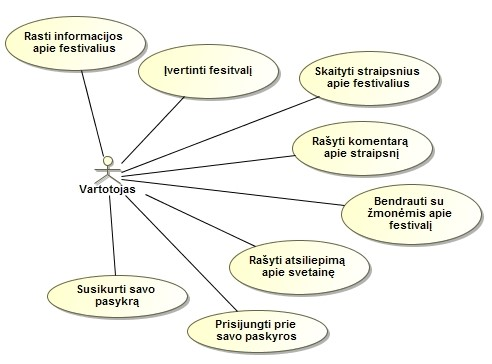
\includegraphics[scale=0.5]{img/Pav/Vartotojas}
    \label{img:uml1}
	\caption{Vartotojo užduotys}
\end{figure}

Vartotojas gali prisiregistruoti prie mūsų tinklalapio. Kad tai padarytų jam reikia atsidarius tinklalapį jo viršuje paspausti registracijos mygtuką, tada yra pateikiama registracijos formą, kurią jis privalo užpildyti. Ji yra išsiunčiama registracijos kontrolei, kuri išsaugo naują vartotoją duomenų bazėje. Ji atsako ar yra jau toks vartotojo vardas.  Jeigu toks vardas neegzistuoja, yra atidaroma vartotojo paskyrą, o jei toks vartotojo vardas egzistuoja tinklalapis vartotojui praneša, kad yra suvesti negalimi registracijos duomenys.

\begin{figure}[H]
    \centering
    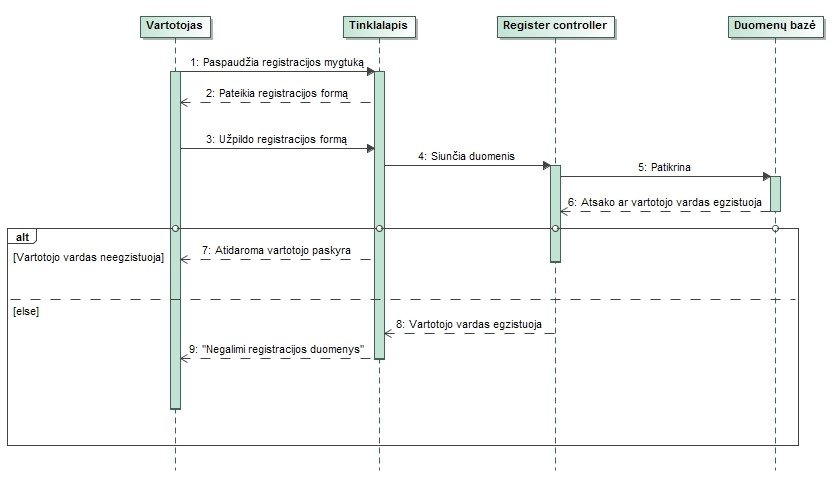
\includegraphics[scale=0.5]{img/Pav/VartotojoRegistracija}
    \label{img:uml2}
	\caption{Vartotojo registracijos seka}
\end{figure}

Vartotojas gali prisijungti prie tinklalapio. Kad tai padaryti vartotojas turi tinklalapio viršuje paspausti prisijungimo mygtuką. Tai padarius atsiveria prisijungimo langas, kurį užpildžius duomenys yra išsiunčiami į prisijungimo vadovą. Jis pateikia duomenis duomenų bazei patikrinti ar vartotojas egzistuoja. Jeigu toks vartotojas egzistuoja jam yra atidaroma jo paskyra, o jeigu tokio vartotojo nėra pranešama, kad vartotojas neegzistuoja su tokiais duomenimis.

\begin{figure}[H]
    \centering
    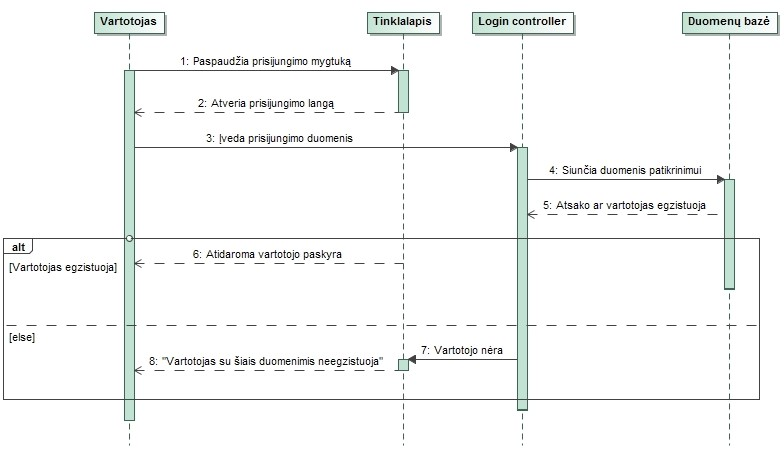
\includegraphics[scale=0.5]{img/Pav/VartotojoPrisijungimas}
    \label{img:uml3}
	\caption{Vartotojo prisijungimo seka}
\end{figure}

Vartotojas gali peržiūrėti festivalių sąrašą. Jis turi atsidaryti tinklalapį pasirinkti skiltį “Festivaliai”, tuomet tinklalapis prašo imti festivalių sąrašą iš vartotojo valdovo ( ang. User controller), kuris paima informaciją iš DB. Tada vartotojo valdovas siunčia informaciją tinklalapiui, kuris ją atvaizduoja vartotojui.
Jeigu vartotojas nori daugiau informacijos apie festivalį, jis turi pasirinkti festivalį. Tada jo ID yra siunčiama vartotojo valdovui, kuris iš DB paima to festivalio informaciją ir tada ją siunčia tinklalapiui. Šis atidaro naują langą su visa informacija. Taip pat, vartotojas gali rašyti komentarus  prie festivalių arba juos vertinti. Tačiau tai gali daryti tik prisijungę vartotojai. Jeigu vartotojas yra prisijungęs jam yra leidžiama naudotis festivalio komentarų bei vertinimo erdve, tada jis gali parašyti komentarą arba vertinimą, kuriuos siunčia į vartotojo vadovą, kuris komentarą arba vertinimą saugo į DB. Vartotojo vadovas patvirtina, kad duomenys yra įkelti. Ir tada tinklalapyje atsiranda komentaras arba vertinimas. Tačiau jeigu vartotojas neturi paskyros jam tinklalapis rašo, kad norint komentuoti arba vertinti reikia turėti paskyrą.

\begin{figure}[H]
    \centering
    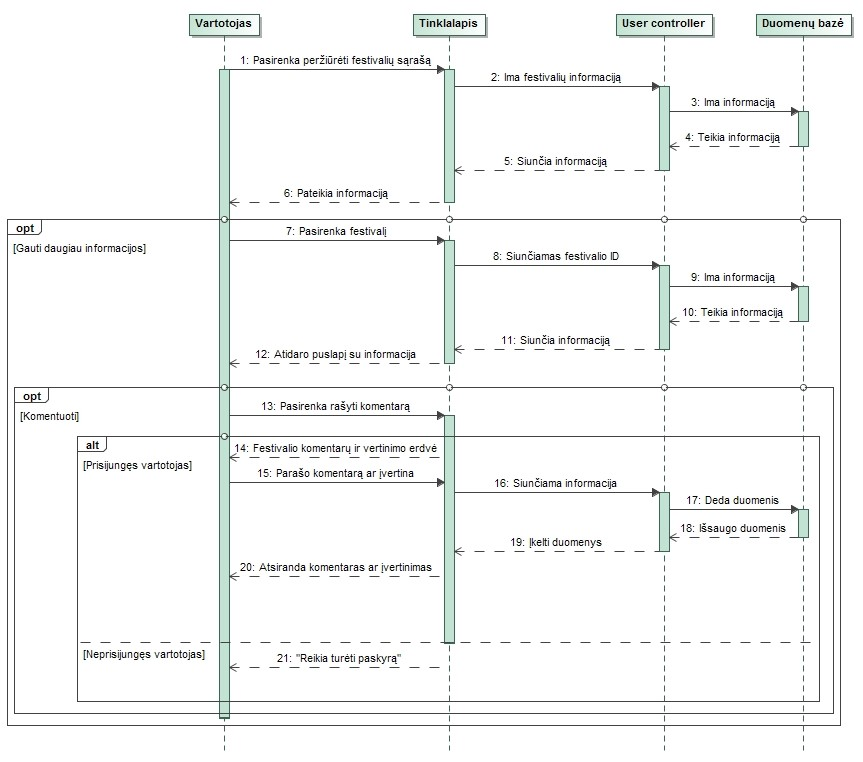
\includegraphics[scale=0.5]{img/Pav/VartotojoInfoFest_Komentarai}
    \label{img:uml4}
	\caption{Vartotojo veiksmai su festivaliais}
\end{figure}

Vartotojas gali peržiūrėti visus straipsnius. Tai gali padaryti atsidarydamas tinklalapį ir pasirinkdamas skiltį “Naujienos”. Tada tinklalapis siunčia prašymą vartotojo vadovui, kuris iš duomenų bazės ima informaciją ir ją siunčia į tinklalapį, kuris ją pateikia vartotojui. Jeigu vartotojas nori perskaityti visą straipsnį, spaudžia “Skaityti daugiau” ir tada tinklalapis siunčia straipsnio ID vartotojo vadovui, kuris ima informaciją apie tą straipsnį ir jį siunčia į tinklalapį, kuris naujame puslapyje vartotojui parodo straipsnį.
	Beje, jei vartotojas yra prisijungęs jis gali rašyti komentarą. Šis komentaras yra siunčiamas vartotojo vadovui, kuris įkelia komentarą į DB. Tada, vartotojo vadovas tinklalapiui praneša apie sėkmingą išsaugojimą ir tinklalapyje atsiranda komentaras. Tačiau jei vartotojas nėra prisijungęs tinklalapis jam praneša, kad reikia būti prisijungusiam.

\begin{figure}[H]
    \centering
    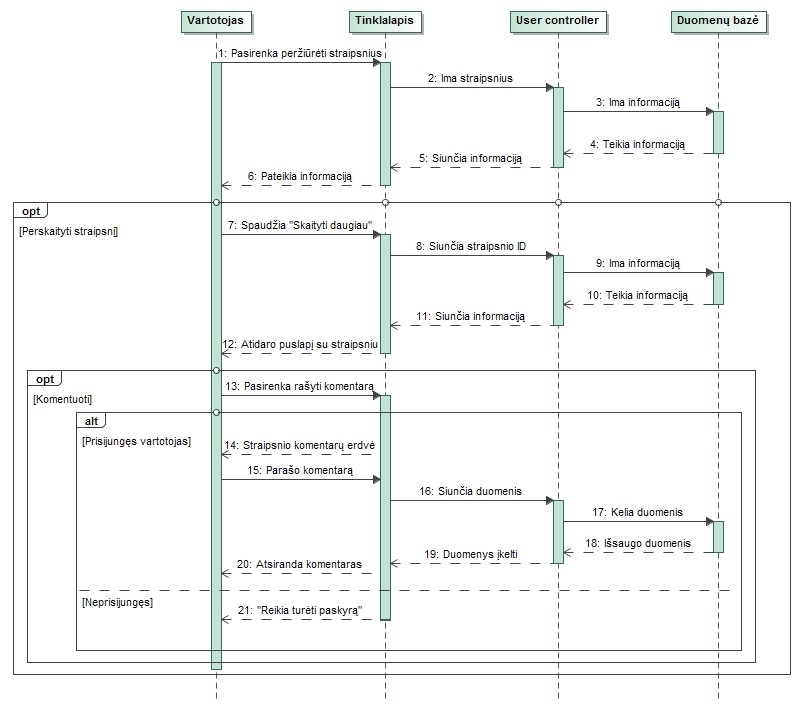
\includegraphics[scale=0.5]{img/Pav/VartotojasStraips_Komentarai}
    \label{img:uml5}
	\caption{Vartotojo veiksmai su straipsniais}
\end{figure}	
	
Vartotojas gali parašyti atsiliepimą. Tai padaryti jis gali atsidaręs tinklalapį ir pasirinkęs skiltį “Apie mus”. Ten jis parašo atsiliepimą, kuris su vartotojo ID yra siunčiami vartotojo vadovui, kuris saugo informaciją į DB. Ir kai saugojimas yra įvykdytas vartotojo vadovas praneša apie sėkmingą įkėlimą tinklalapiui, kuris informuoja vartotoją. Kadangi yra reikalingas ir vartotojo ID, atsiliepimus gali rašyti tik prisijungę vartotojai.
	
\begin{figure}[H]
    \centering
    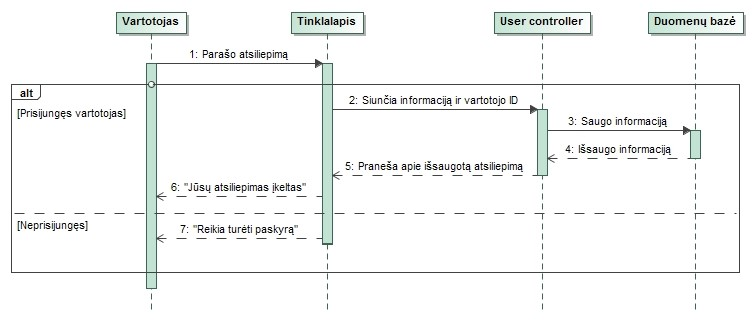
\includegraphics[scale=0.5]{img/Pav/VartotojasAtsiliepimas}
    \label{img:uml6}
	\caption{Vartotojo atsiliepimų seka}
\end{figure}	
	
Sekantis agentas yra festivalio organizatorius su vienu tikslu.

\begin{figure}[H]
    \centering
    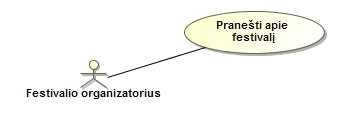
\includegraphics[scale=0.5]{img/Pav/FestivalioOrg}
    \label{img:uml7}
	\caption{Festivalio organizatoriaus užduotis}
\end{figure}	
	
Festivalio organizatorius gali atlikti tik vieną užduotį. Tai yra pranešti apie festivalį. Jis tai gali padaryti atsidaręs tinklalapį ir pasirinkęs skiltį “Festivaliai” ir ten paspaudęs ant mygtuko “Pranešti apie festivalį”. Tuomet tinklalapis pateikia festivalio formą, kurią festivalio organizatorius užpildo ir visa informacija yra išsiunčiama į Admin panel.

\begin{figure}[H]
    \centering
    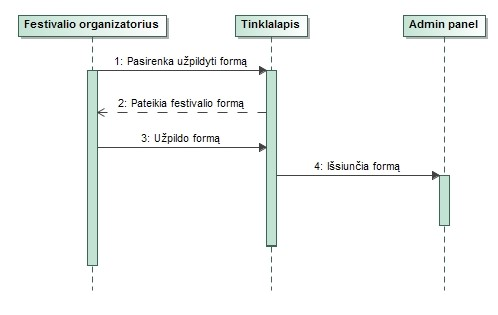
\includegraphics[scale=0.5]{img/Pav/FestivalOrgPranesti}
    \label{img:uml8}
	\caption{Festivalio organizatoriaus veiksmų seka}
\end{figure}	

Dar vienas agentas yra administratorius su daugiausia užduočių mūsų tinklalapyje. Jis paveldi visas žurnalisto užduotis.

\begin{figure}[H]
    \centering
    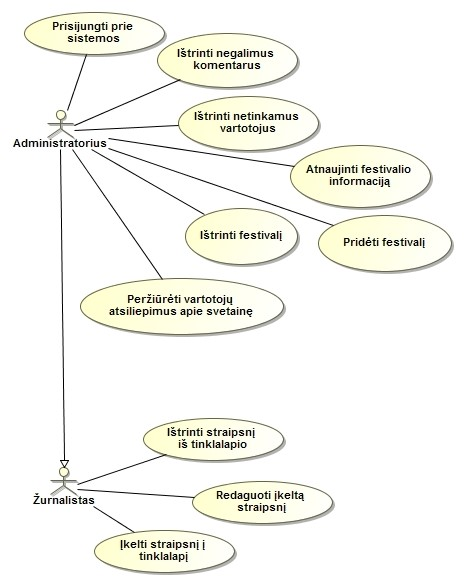
\includegraphics[scale=0.6]{img/Pav/Administratorius}
    \label{img:uml9}
	\caption{Administratoriaus užduotys}
\end{figure}	

Administratorius gali prisijungti prie sistemos. Tai padaryti jis gali, kai užpildo prisijungimo formą, kurią pateikia admin panel. Ji prisijungimo duomenis siunčia DB vadovui (ang. DB controller), kuris juos tikrina DB’ėje. Jeigu duomeys yra tinkami yra leidžiama naudotis admin panel, o jeigu duomenys nėra rasti - pranešama, kad tokių duomenų nėra sistemoje.

\begin{figure}[H]
    \centering
    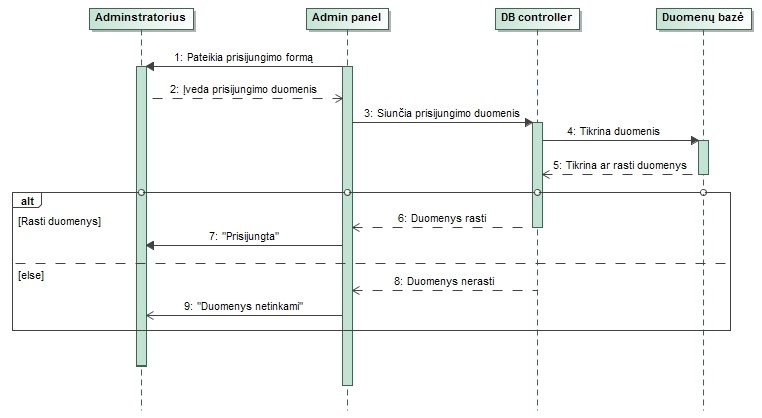
\includegraphics[scale=0.5]{img/Pav/AdminPrisijungtiPrieSis}
    \label{img:uml10}
	\caption{Administratoriaus prisijungimo veiksmų seka}
\end{figure}

Administratorius gali pridėti festivalį, kurį atsiuntė į sistemą festivalio organizatorius. Jis tai gali padaryti paspaudęs mygtuką “Pridėti festivalį”, tuomet admin panel pateikia festivalio formą, kurią administratorius užpildo pagal atsiųsta informaciją. Tuomet ta informacija yra siunčiama DB vadovui, kuris ją išsaugo DB ir įkelia tą festivalį į tinklalapį bei praneša admin panel apie sėkmingą įkėlimą, o ši informuoja administratorių.

\begin{figure}[H]
    \centering
    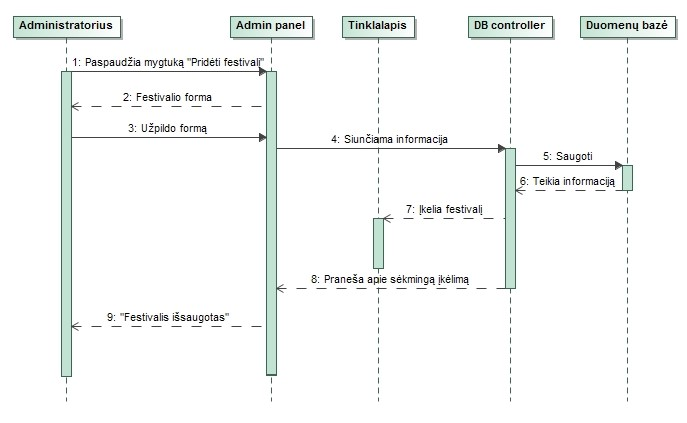
\includegraphics[scale=0.5]{img/Pav/AdminPridetiFestivali}
    \label{img:uml11}
	\caption{Administratorius prideda festivalį}
\end{figure}
	
Administratorius gali peržiūrėti visus publikuotų festivalių skelbimus. Tai gali padaryti pasirinkęs peržiūrėti festivių sąrašą. Tada, admin panel prašo gauti informacijos DB vadovui, o jis iš DB ima ir siunčia informaciją admin panel, kad ji informaciją pateiktų administratoriui. Tada administratorius gali pasirinkti festivalį ir padaryti tokius pasirinkimus: 
\begin{itemize}
\item Ištrinti festivalį. Tada admin panel nusiunčia festivalio ID DB vadovui, kuris ištrina festivalį iš DB ir praneša apie sėkmingą funkcijos atlikimą. Ir admin panel praneša administratoriui apie festivalio ištrinimą;
\item Atnaujinti festivalį. Tada yra nusiunčiamas festivalio ID ir DB vadovas gauna informaciją iš DB ir ją siunčia į admin panel, kuri pateikią festivalio informacijos forma administratoriui. Tuomet administratorius gali pakeisti to festivalio infromaciją ir ją išsaugoti. Tada admin panel siunčia informaciją DB vadovui, kuris atnaujina informaciją DB ir praneša apie sėkmingą atnaujinimą, o admin panel praneša apie tai administratoriui. 
\end{itemize}
	
\begin{figure}[H]
    \centering
    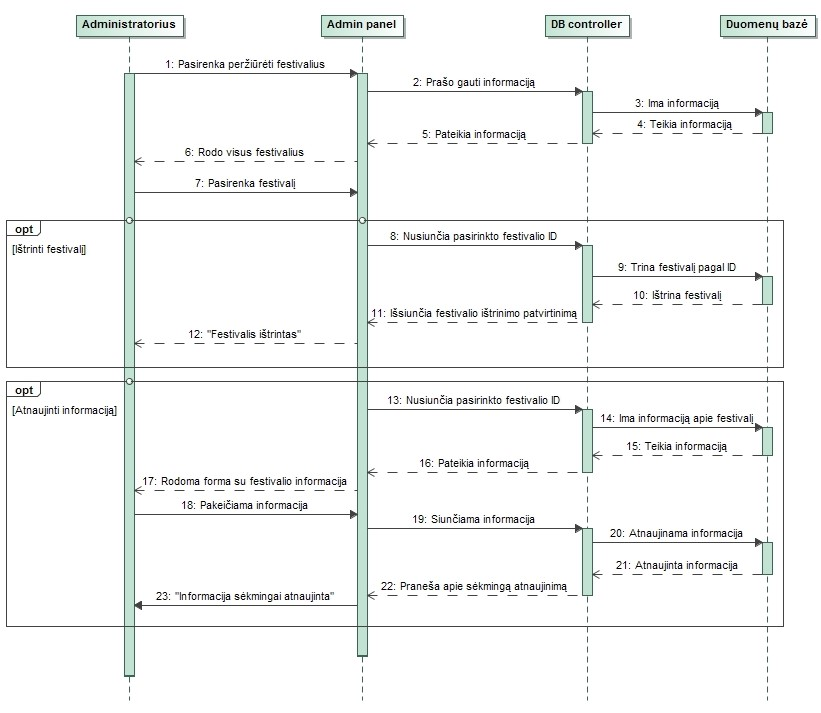
\includegraphics[scale=0.5]{img/Pav/AdminIstrintiAtnaujintiFest}
    \label{img:uml12}
	\caption{Administratorius veiksmai su festivaliais}
\end{figure}	
	
Administratorius gali ištrinti vartotojus, kurie pastoviai nusižengia tinklalapio taisyklėms. Tai jis gali padaryti pasirinkdamas, kad jam parodytų vartotojų sąrašą. Admin panel prašo dauti informacijos DB vadovo, o šis ima informaciją iš DB ir ją siunčia atgal į admin panel. O admin panel pateikia sąrašą administratoriui. Jis gali pasirinkti vartotoją. Tada to vartotojo ID yra siunčiamas DB vadovui, kuris paima to vartotojo informaciją iš DB ir ją siunčia į admin panel. Tada admin panel atidaro naują langą su visa statistine informaciją apie vartotoją. Jeigu administratorius nusprendžia, kad vartotoją reikia ištrinti jis pasirenka tokia funkciją ir admin panel išsiunčia to vartotojo ID DB vadovui, kuris pašalina iš DB tą vartotoją ir visą informaciją su juo bei gražina, kad funkcija sėkmingai įvykdyta.

\begin{figure}[H]
    \centering
    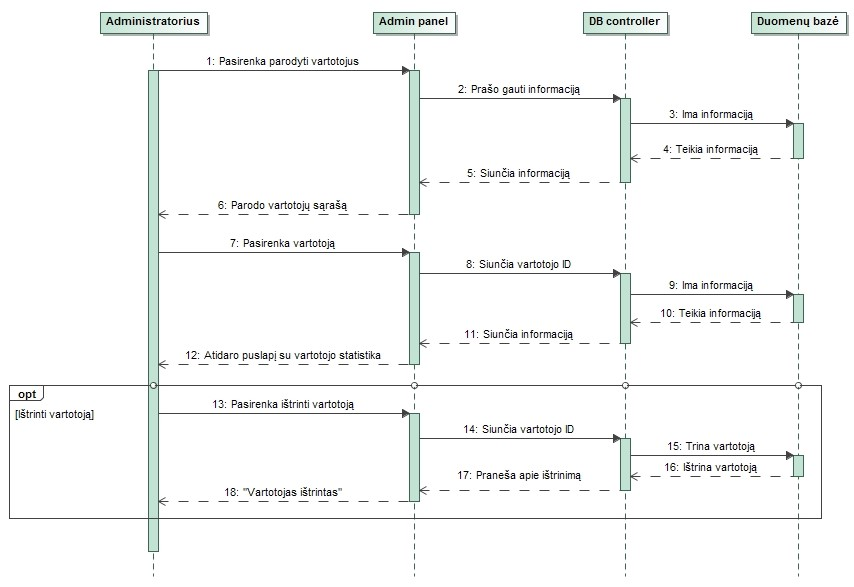
\includegraphics[scale=0.5]{img/Pav/AdminIstrintiVartotoja}
    \label{img:uml13}
	\caption{Administratorius ištrina vartotoją}
\end{figure}	
	
Administratorius gali ištrinti netinkamą komentarą. Tai padaryti jis gali, kai pasirenka, kad jam admin panel rodytų visus komentarus bei gali pasirinkti pagal ką jam bus rodomi komentarai: nauji nuo paskutinio patikrinimo, nuo tam tikros datos ar tam tikro festivalio (straipsnio) ir t.t.. Tada admin panel prašo gauti informaciją DB vadovo, jis paima informaciją iš DB ir siunčia į admin panel, kuri sąrašą atvaizduoją administratoriui. Kai administratorius pasirenka komentarą, admin panel siunčia to komentaro ID DB vadovui ir šis iš DB ištrina tą komentarą bei praneša apie sėkmingą ištrinimą. Admin panel parodo pranešimą, kad komentaras ištrintas, administratoriui. 
	Tačiau administratorius gali peržvelgti tik tuos komentarus, kuriuos pranešė kiti vartotojai. Jis pasirenka šia opciją ir admin panel prašo DB vadovo, kad duotų informacijos ir šis paima ją iš DB ir siunčia admin panel, kuri administratoriui juos parodo. Tada administratorius pasirenka netinkamus ir ištrina. Admin panel siunčia komentarų ID ir DB vadovas juos ištrina iš DB ir praneša apie sėkimingą funkcijos įvykdymą.

\begin{figure}[H]
    \centering
    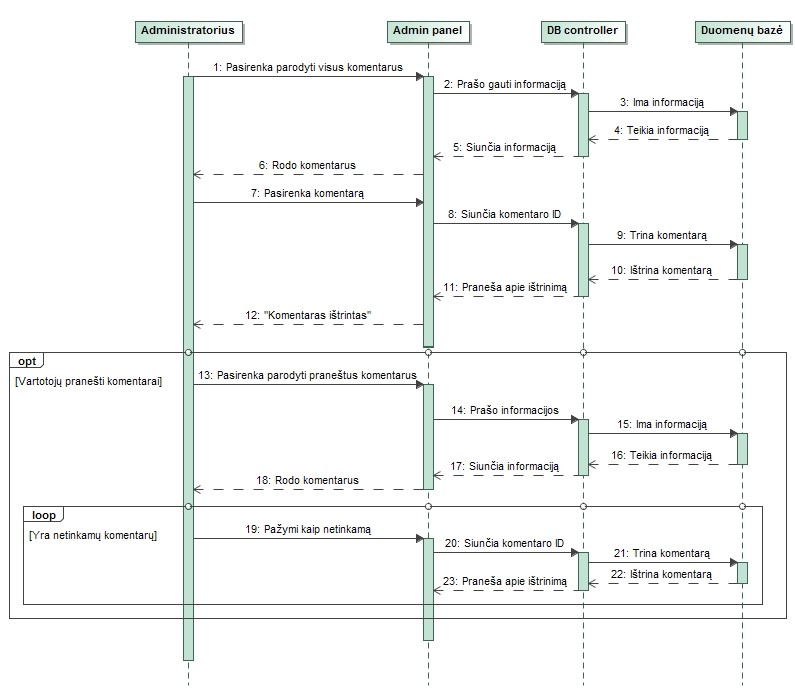
\includegraphics[scale=0.5]{img/Pav/AdminIstrintiKomentarus}
    \label{img:uml14}
	\caption{Administratorius ištrina komentarą}
\end{figure}	
	
Administratorius gali peržiūrėti visus vartotojų atsiliepimus. Jis turi pasirinkti tokią opciją ir tada admin panel prašo DB vadovo suteikti tokią informaciją. Tada DB vadovas paima informaciją iš DB ir ją išsiunčia į admin panel, kuri šią informaciją atvaizduoja. Tada, administratorius gali ištrinti bereikšmius atsiliepimus iš sistemos. Jis turi pasirinkti atsiliepimą, tada to atsiliepimo ID yra išsiunčiamas DB vadovui, kuris ištrina atsiliepimą iš DB ir praneša apie sėkmingą to atlikimą. Ir tada admin panel apie tai praneša administratoriui.
	
\begin{figure}[H]
    \centering
    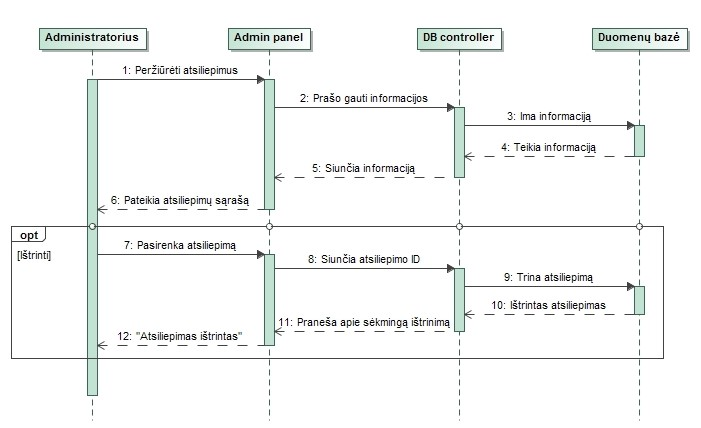
\includegraphics[scale=0.5]{img/Pav/AdminAtsiliepimaiSvetaine}
    \label{img:uml15}
	\caption{Administratorius peržiūri atsiliepimus}
\end{figure}
	
Paskutinis agentas mūsų tinklalapyje yra žurnalistas, kurio užduotis turi ir administratorius.

Žurnalistas gali įkelti straipsnį į tinklalapį. Tai padaro pasirinkdamas įkelti straipsnį, tada zurnalistas panel pateikia straipsnio formą, kurią žurnalistas užpildęs deda į sistemą. Zurnalistas panel siunčia informaciją DB vadovui, kuris saugo informaciją į DB ir taip pat ima informaciją iš DB tam, kad galėtų automatiškai įkelti į tinklalapį. O apie sėkmingą įkėlimą zurnalistas panel praneša žurnalistui.

\begin{figure}[H]
    \centering
    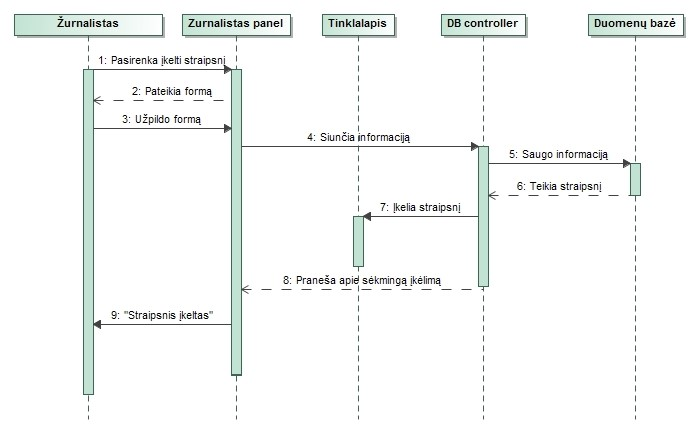
\includegraphics[scale=0.5]{img/Pav/ZurnalistasIkeliaStraipsni}
    \label{img:uml16}
	\caption{Žurnalistas įkelia straipsnį}
\end{figure}

Žurnalistas gali ir peržvelgti visus straipsnius. Kai žurnalistas pasirenka tokią galimybę zurnalistas panel prašo informacijos DB vadovo, kuris ją ima iš DB ir siunčia atgal į zurnalistas panel, o ši pateikia sąrašą žurnalistui. Tada žurnalistas pasirenka straipsnį ir jis gali pasirinkti ką, daryti:
\begin{itemize}
\item Ištrinti. Tada zurnalistas panel siunčia straipsnio ID DB vadovui, kuris ištrina straipsnį iš DB ir praneša apie sėkmingą ištrinimą. O zurnalistas panel praneša apie straipsio ištrinimą žurnalistui.
\item Redaguoti. Zurnalistas panel siunčia straipsnio ID DB vadovui, kuris ima informaciją iš DB ir ją siunčia į zurnalistas panel, kuri straipsnio formą pateikia žurnalistui. Jis gali redaguoti visą straipsnio informaciją, o baigęs išsaugoti. Tada zurnalistas panel siunčia informaciją DB vadovui, kuris atnaujina straipsnio informaciją ir apie sėkmingą atnaujinimą praneša. O zurnalistas panel praneša apie sėkmingą atnaujinimą žurnalistui.
\end{itemize}	
	
\begin{figure}[H]
    \centering
    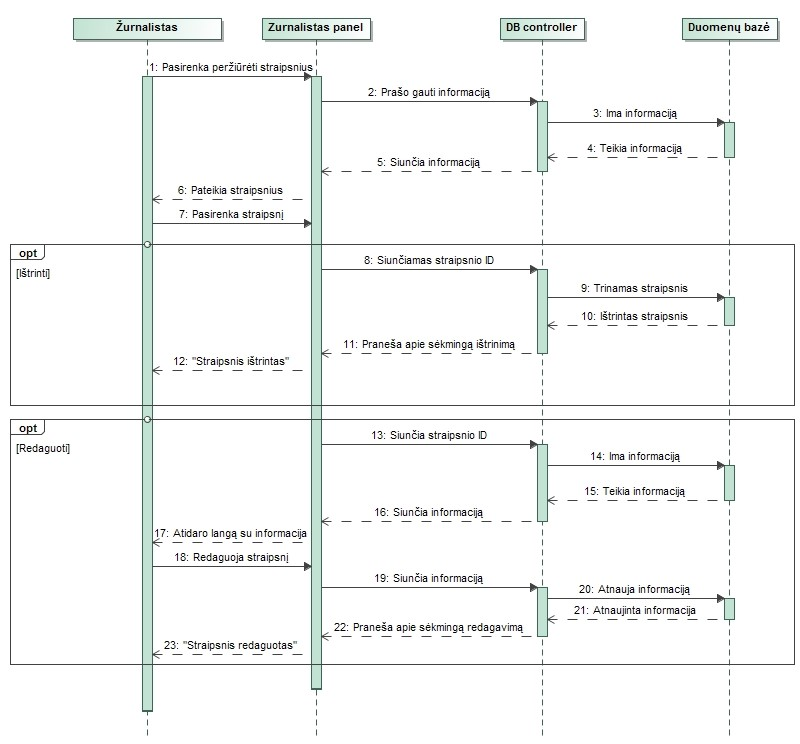
\includegraphics[scale=0.5]{img/Pav/ZurnalistasIstrina_Redaguoja}
    \label{img:uml16}
	\caption{Žurnalisto atliekamų veiksmų sekos}
\end{figure}	
	
\section{Struktūrinis programų sistemos modelis}
Šiame skyriuje nagrinėjamas funkcinių reikalavimų įgyvendinimas, vaizduojamos informacinę festivalių sistemą sudarančios klasės ir jų sąryšiai.

Pirmiausiai pateikiama UML paketų diagrama, kurioje vaizduojamos viso klasės ir jų skirstymas į paketus.
\begin{figure}[H]
\centering
    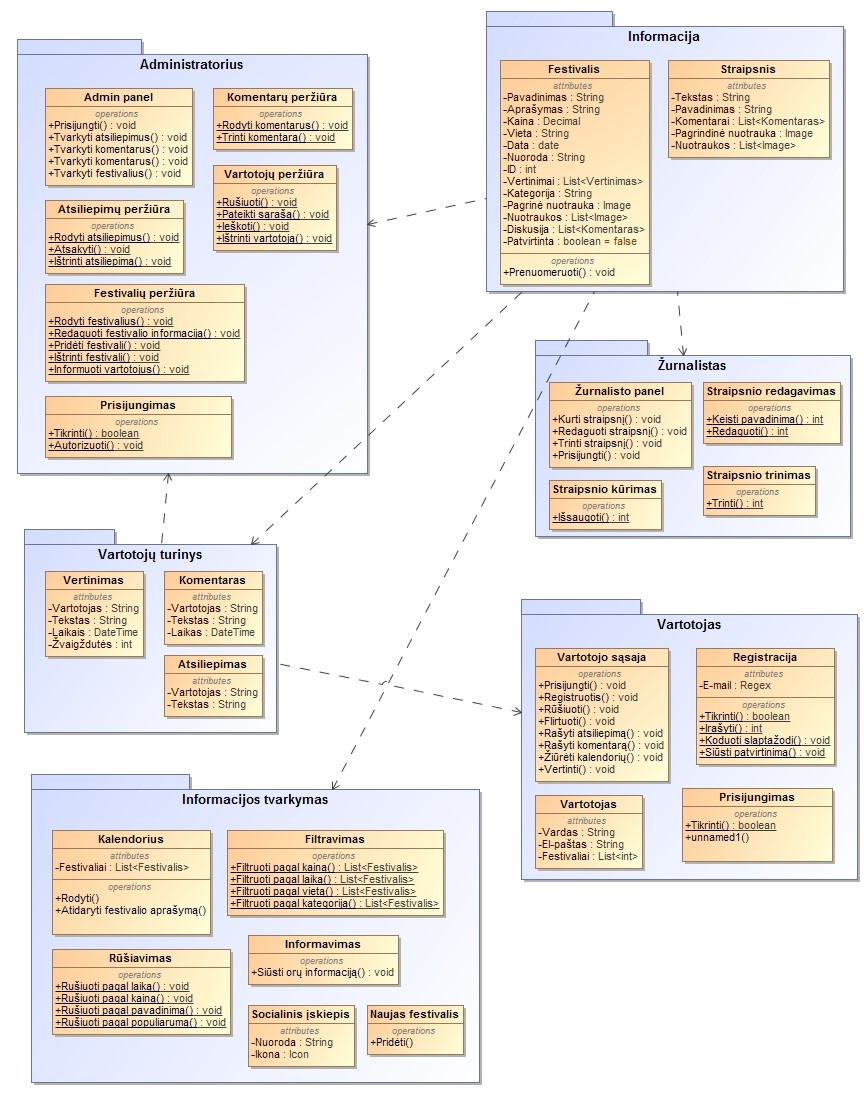
\includegraphics[scale=0.5]{img/PSI3/paketai}
	\label{img:uml17}
	\caption{Klasių skirstymas į paketus}
\end{figure}
\newpage
Toliau pateiktoje klasių diagramoje vaizduojami klasių, apibrėžiančių administratoriui skirtas funkcijas, ryšiai. \textit{Admin panel} klasė paveldi iš \textit{Žurnalisto panel} klasės, nes ir administratorius gali atlikti visas žurnalisto užduotis.
\begin{figure}[H]
\centering
    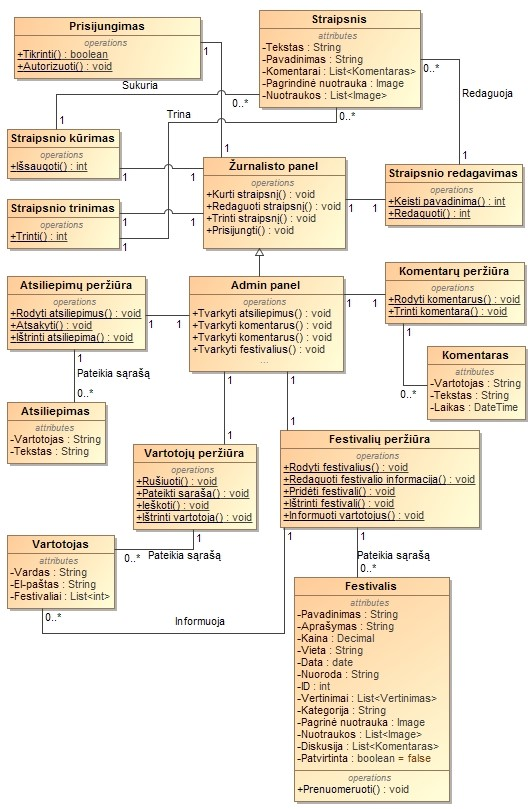
\includegraphics[scale=0.65]{img/PSI3/admin}
	\label{img:uml18}
	\caption{Klasės, leidžiančios atlikti administratoriaus funkcijas}
\end{figure}
Pagrindinė klasė, leidžianti atlikti žurnalisto užduotis, yra \textit{Žurnalisto panel}. \textit{Žurnalisto panel} naudoja klases: \textit{Straipsnio kūrimas, Straipsnio redagavimas, Straipsnio trynimas}. Šios klasės turi prieigą prie duomenų bazėje saugomų straipsnių, todėl yra susijusios su klase \textit{Straipsnis}. \textit{Žurnalisto panel} taip pat naudoja klasę \textit{Prisijungimas}.
Pagrindinė klasė, leidžianti atlikti administratoriaus užduotis, yra \textit{Admin panel}. Be klasių, kurias naudoja \textit{Žurnalisto panel} klasė, \textit{Admin panel} naudoja klases: \textit{Atsiliepimų peržiūra, Vartotojų peržiūra, Komentarų peržiūra, Festivalių peržiūra}. Kadangi šiose klasėse yra metodai leidžiantys dirbti su duomenų bazėje saugoma informacija, klasė \textit{Atsiliepimų peržiūra} yra susijusi su klase \textit{Atsiliepimas}, \textit{Vartotojų peržiūra} - su \textit{Vartotojas}, \textit{Komentarų peržiūra} - su \textit{Komentaras} bei \textit{Festivalių peržiūra} - su \textit{Festivalis}. \textit{Festivalių peržiūra} yra susijusi su klase \textit{Vartotojas}, nes klasėje \textit{Festivalių peržiūra} yra metodas, leidžiantis siūsti informaciją visiem tam tikrą festivalį užsiprenumeravusiems vartotojams.

Žemiau pateiktoje diagramoje vaizduojamas klasių, leidžiančių informuoti vartotoją apie oro sąlygas likus trim dienom iki festivalio, sąryšis.
\begin{figure}[H]
\centering
    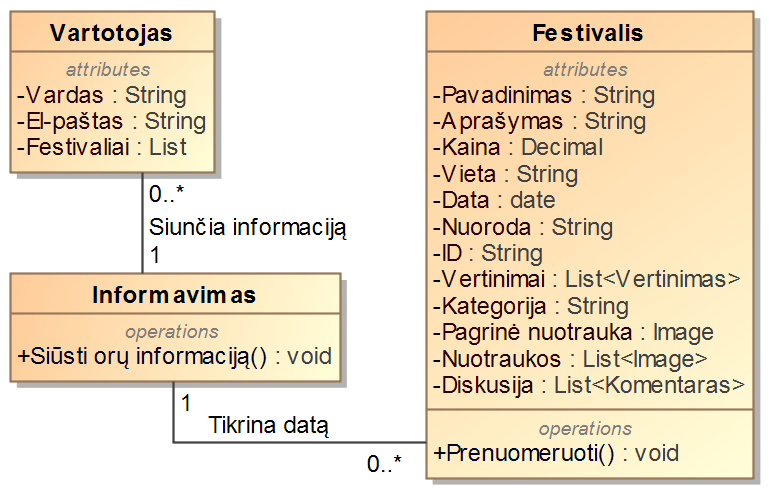
\includegraphics[scale=0.45]{img/PSI3/orai.PNG}
	\label{uml:19}
	\caption{Klasės, leidžiančios informuoti vartotoją}
\end{figure}
Klasė \textit{Informavimas} yra susijusi su klase \textit{Festivalis}, nes tikrina festivalių datas. Kadangi klasė \textit{Informavimas} turi metodą, leidžiantį siųsti informaciją vartotojams, yra susijusi su klase \textit{Vartotojas}.

Toliau pateikiama naujo festivalio įtraukimo į duomenų bazę diagrama.
\begin{figure}[H]
\centering
    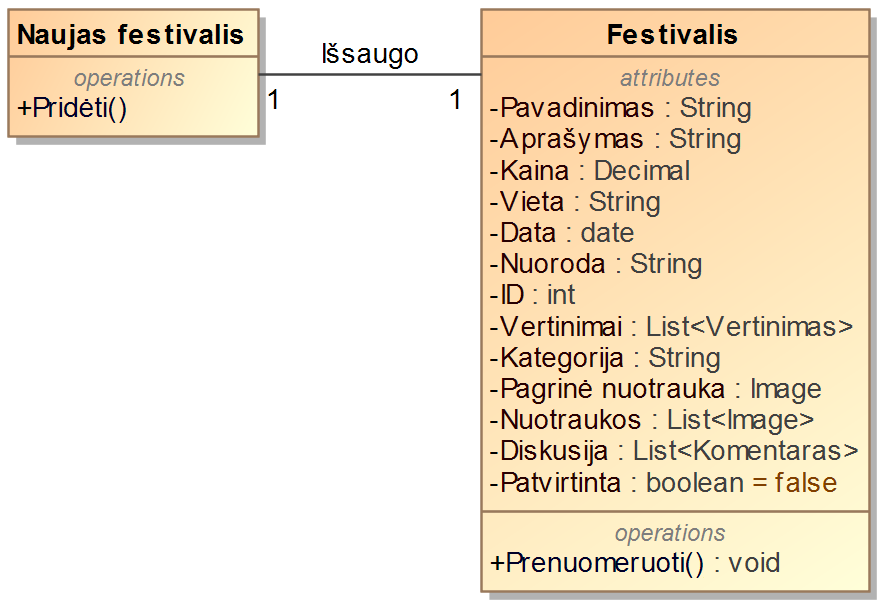
\includegraphics[scale=0.45]{img/PSI3/naujas.PNG}
	\label{uml:20}
	\caption{Klasės, leidžiančios įkelti informaviją apie nauja festivalį}
\end{figure}
Kai užpildoma anketa apie naują festivalį, naujas \textit{Festivalis} yra įtraukiamas į duomenų bazę. Kol administrsatorius nepatikrina pateiktos informacijos \textit{Patvirtinta} turi vertę \textit{false}.

Toliau pateiktoje klasių diagramoje vaizduojami klasių, apibrėžiančių vartotojui skirtas funkcijas, ryšiai.
\begin{figure}[H]
\centering
    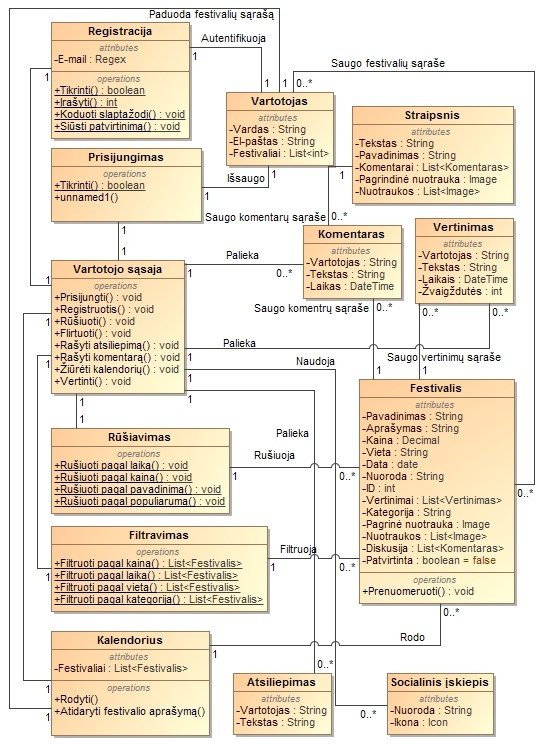
\includegraphics[scale=0.65]{img/PSI3/user}
	\label{uml:21}
	\caption{Klasės, leidžiančios atlikti vartotojo funkcijas}
\end{figure}
Pagrindinė klasė, leidžianti atlikti vartotojo užduotis, yra \textit{Vartotojo sąsaja}. \textit{Vartotojo sąsaja} yra susijusi su klasėmis: \textit{Prisijungimas, Registracija, Kalendorius, Rūšiavimas, Filtravimas, Socialinis įskiepis, Komentaras, Vertinimas, Atsiliepimas}. Klasė \textit{Prisijungimas} gali tikrinti vartotojų sąrašą, o \textit{Registracija} - pridėti naujus vartotojus, todėl šios klasės yra susijusios su klase \textit{Vartotojas}. Klasė \textit{Komentaras} yra susijusi su klase \textit{Straipsnis}, nes \textit{Straipsnis} saugo komentarų sąrašą. Klasės \textit{Komentaras} ir \textit{Vertinimas} yra susijusios su klase \textit{Festivalis}, nes \textit{Festivalis} saugo komentarų ir vertinimų sąrašus. Klasė \textit{Kalendorius} yra susijusi su klase \textit{Festivalis}, nes \textit{Kalendorius} saugo vartotojo pasirinktus festivalius. \textit{Kalendorius} turi sąryšį su klase \textit{Vartotojas}, nes atvaizdavimui naudoja vartotojo festivalių sąrašą. Klasės \textit{Rūšiavimas} ir \textit{Filtravimas} yra susijusios su klase \textit{Festivalis}, nes jos pertvarko vartotojui rodomą festivalių sąrašą.

\section{Dinaminis programų sistemos modelis}

Šiame skyrelyje apžvelgsime, kaip tinklalapio veikimo metu veikia aplikacija ir keičiasi kelių jos elementų būsenos. Tai atlikome naudodami veiklos diagramas, pritaikydami jas pagrindiniams tinklalapio procesams, ir būsenos diagramas, pritaikę jas tinklalapiui ir vartotojui.


Žemiau pateikta veiklos diagrama, kuri rodo ką vartotojas gali daryti tinklalapyje pasirinkęs “Festivaliai” skiltį. Vartotojas gali tiesiog ieškoti straipsnio eidamas per visą skiltį arba jis gali tikslingai pasirinkti rikiavimo arba filtravimo būdą, arba žinodamas festivalio pavadinimą - jį gali įvesti į paieškos laukelį. Iš atrinktų festivalių vartotojas gali toliau rinktis festivalį. O tada gali išsirinkti vieną festivalį ir arba jis randa informaciją, kurios ir ieškojo, arba, jeigu vartotojas yra prisijungęs, jis gali įvertinti festivalį, diskutuoti su žmonėmis arba užsiprenumeruoti festivalį. Jeigu vartotojas užsiprenumeruoja festivalį, tada likus trims dienoms iki festivalio jam yra pranešama, kokia bus meteorologinė situacija festivalio metu.

\begin{figure}[H]
	\centering
    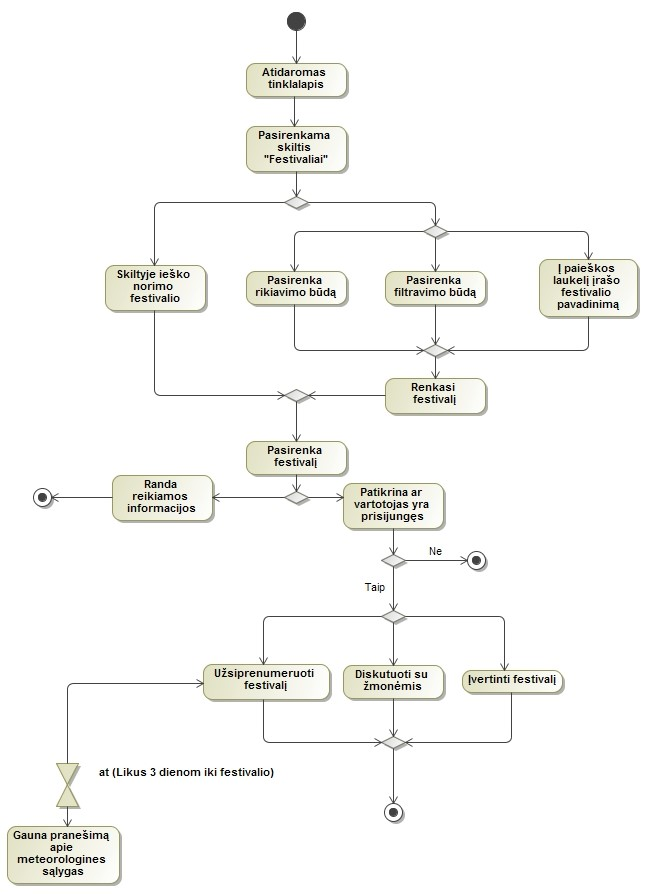
\includegraphics[scale=0.5]{img/Pav/VartotojasFestivalis}
	\label{uml:22}
	\caption{Vartotojo veiksmai "Festivaliai" skiltyje}
\end{figure}

Beje, vartotojas gali pasirinkti skiltį “Naujienos”. Tada jis gali ieškoti straipsnio, jeigu jis randa straipsnį, kurį nori perskaityti - spaudžia “Skaityti daugiau”. Tada gali perskaityti straipsnį ir jeigu nori bei yra prisijungęs vartotojas gali komentuoti. Arba gali eiti toliau ieškoti straipsnio.

\begin{figure}[H]
	\centering
    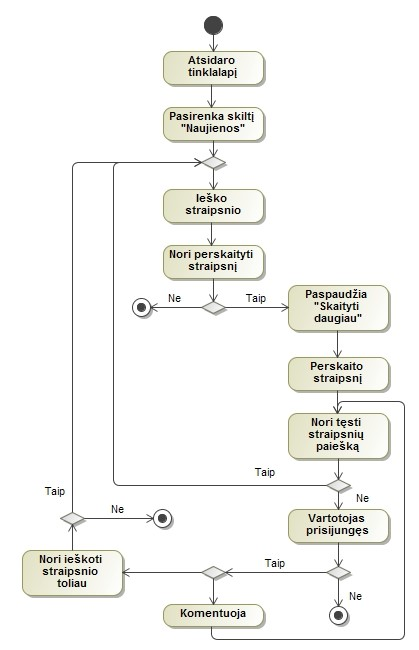
\includegraphics[scale=0.5]{img/Pav/VartotojasStraipsnis}
	\label{uml:23}
	\caption{Vartotojo veiksmai "Naujienos" skiltyje}
\end{figure}

Vartotojas atsidaręs tinklalapį, jei turi paskyrą gali prie jos prisijungti. Tai padaro paspausdamas prisijungimo mygtuką ir įvesdamas prisijungimo duomenis ir taip prisijungia. Tačiau jei jis neturi savo paskyros vartotojas gali paspausti registracijos mygtuką ir tada gali pasirinkti naudoti įskiepius, jeigu nenori jis užpildo registracijos formą, o jeigu nori naudoja įskiepius. Ir taip susikuria paskyrą.
	Prisijungęs ar susikūręs pasykrą vartotojas gali paspausti ant “Mano meniu” mygtuko ir tada gali rinktis ką nori daryti:
\begin{itemize}
\item Gali paspausti ant mygtuko “Mano kalendorius” ir tada pamato jo pasirinktus festivalius kalendoriuje. Jeigu jis nori gauti informacijos vartotojas paspaudžia ant festivalio ir atsiranda langas su festivalio informacija.
\item Gali paspausti ant “Nauji pranešimai” mygtuko ir tada jeigu yra naujų pranešimų jie yra matomi, o jeigu jų nėra, tada būna parašyta, kad naujų pranešimų nėra. 
\item Gali pasirinkti “Užsiprenumeruoti festivaliai” pasirinkties ir tada vartotojas mato sąrašą festivalių, kuriuos jis užsiprenumeravęs. Jeigu nori gali paspausti ant festivalio ir sužinoti daugiau informacijos apie jį.
\item Gali paspausti ant “Nustatymai”. Tada vartotojas gali pakeisti savo paskyros duomenis (slapyvardis, slaptažodis, paskyros paveikslėlį) arba gali pakeisti “Domina” nustatymus.
\end{itemize}
 Visais atvejais vartotojas gali grįžti į “Mano meniu” ir tęsti veiklą.
 
\begin{figure}[H]
	\centering
    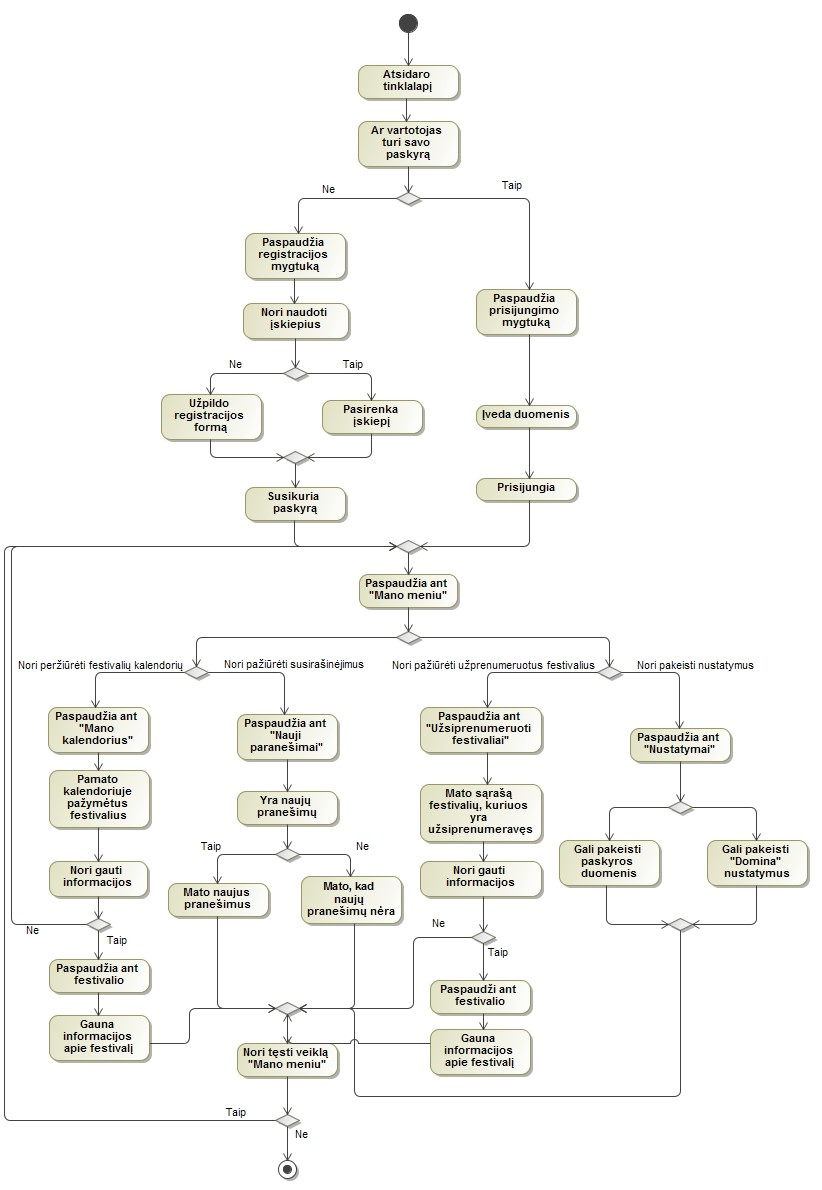
\includegraphics[scale=0.5]{img/Pav/VartotojasPrisijungesFunk}
	\label{uml:24}
	\caption{Vartotojo veiksmai prisijungus}
\end{figure}

Festivalio organizatorius gali pasidalinti savo festivaliu. Jis tai daro pirmiausiai atsidarydamas tinklalapį bei pasirinkdamas skiltį “Festivaliai”. Tada paspaudžia ant mygtuko “Pranešti apie festivalį”. Tada atsidaro naujas puslapis su festivalio formą, kurią užpildęs festivalio organizatorius, ją išsiunčia. Jeigu jis gauna pranešimą, kad reikia patikslinti informaciją turi viską kartoti iš naujo, o jeigu ne, tada festivalio skelbimas išsiųstas.

\begin{figure}[H]
	\centering
    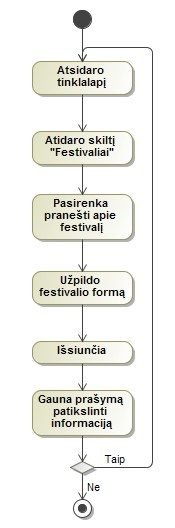
\includegraphics[scale=0.5]{img/Pav/FestOrgFestivalis}
	\label{uml:25}
	\caption{Festivalio organizatorius pasidalina festivaliu}
\end{figure}

Administratorius prisijungęs prie savo admin panel gali daryti keletą veiksmų:
\begin{itemize}
\item Gali pasirinkti pridėti festivalį. Jis pagal festivalio organizatoriaus formą, turi užpildyti festivalio formą ir jeigu informacija teisinga festivalis pridėtas prie sistemos, o jeigu ne, tada išsiunčiamas pranešimas, kad reikia patikslinti informaciją.
\item Gali pasirinkti festivalį ir atnaujinti jo informaciją. Administratorius pasirenka festivalį, pakeičia jo informaciją ir išsaugo atgal į duomenų bazę.
\item Pasirenka ištrinti festivalį. Tada jis pasirenka kokį festivalį reikia ištrinti ir jį ištrina.
Padaręs bet kokį veiksmą administratorius gali toliau tęsti darbą su festivaliais.
\end{itemize}

\begin{figure}[H]
	\centering
    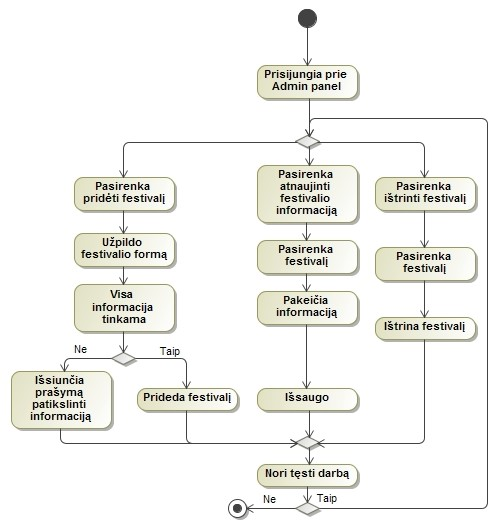
\includegraphics[scale=0.5]{img/Pav/AdminFest}
	\label{uml:26}
	\caption{Administratoriaus veiksmai admin panel su festivaliais}
\end{figure}

Administratorius prisijungęs prie savo admin panel gali daryti keletą veiksmų:
\begin{itemize}
\item Gali pasirinkti ištrinti komentarą. Tada turi pasirinkti ar nori matyti visus ar tik kitų vartotojų praneštus. Tada pasirenka komentarą, peržiūri jo turinį ir nusprendžia ar komentaras yra tinkamas, jeigu netinkamas, tada ištrina komentarą. Ir tada turi pasirinkti ar nori tęsti darbą su komentarais, jeigu taip tada grįžta atgal.
\item Gali pasirinkti ištrinti vartotoją. Tada mato visų vartotojų sąrašą ir pasirenka vartotoją, atsidaro to vartotojo veiklos statistika naujame lange. Jeigu vartotojas nėra geras jis būna ištrinamas. Ir jei administratorius nori gali tęsti darbą su vartotojais.
\item Gali pasirinkti peržiūrėti atsiliepimus. Administratorius peržiūri atsiliepimus, gali pasirinkti atsiliepimą ir jį perskaityti. Tada turi nuspręsti ar atsiliepimas yra tinkamas - jeigu taip, tada padaro pakeitimą pagal vartotojo atsiliepimą, o jeigu ne, tada ištrina atsiliepimą. Jeigu administratorius nori, gali tęsti darbą su atsiliepimais.
\end{itemize}
Visais atvejais administratorius atlikęs veiksmą norėdamas pereiti prie kitos veiklos tai gali padaryti ir tęsti darbą.

\begin{figure}[H]
	\centering
    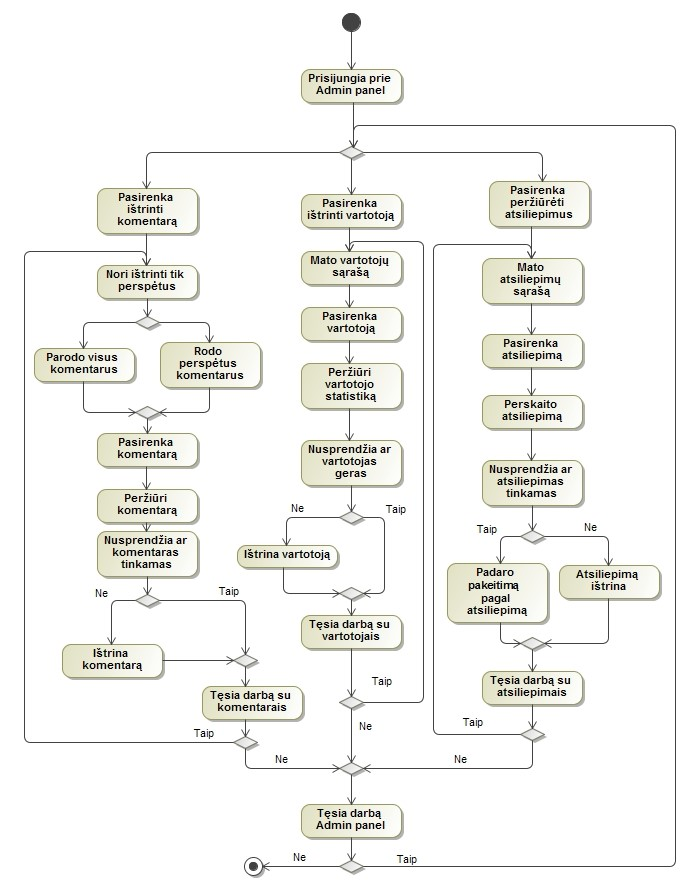
\includegraphics[scale=0.5]{img/Pav/AdminFunkOthers}
	\label{uml:27}
	\caption{Kiti administratoriaus veiksmai admin panel}
\end{figure}

Žurnalistas gali prisijungti prie zurnalistas panel ir gali daryti tokius veiksmus:
\begin{itemize}
\item Gali pasirinkti įkelti naują straipsnį. Tada jis turi užpildyti straipsnio formą ir ją įkelti.
\item Gali pasirinkti redaguoti straipnsį. Tada turi peržiūrėti straipsnių sąrašą ir išsirinkti straipsnį, ant jo paspausti ir tada gavęs jo informaciją gali ją redaguoti. Pabaigęs redagavimą turi išsaugoti.
\item Gali pasirinkti ištrinti straipsnį. Peržvelgęs straipnsių sąrašą jis pasirenka straipsnį ir jį ištrina.
\end{itemize}
Visais atvejais žurnalistas gali toliau tęsti savo darbą.

\begin{figure}[H]
	\centering
    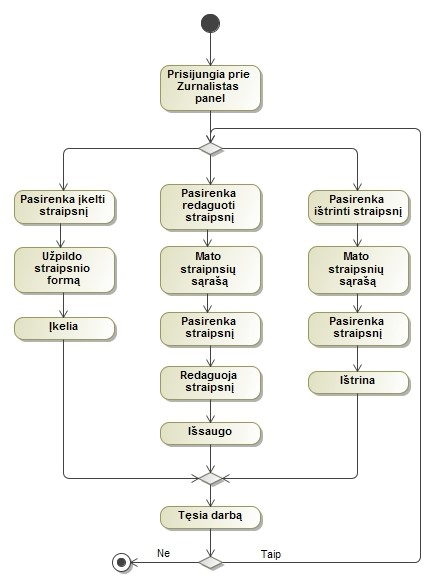
\includegraphics[scale=0.5]{img/Pav/ZurnalistasStraipsniai}
	\label{uml:28}
	\caption{Žurnalisto veiksmai}
\end{figure}

Tinklalapis gali būti: kuriamas, veikiantis, neveikiantis, taisomas, uždarytas. Jeigu tinklalapis neveikia dėl serverio talpintojų problemų arba dėl sistemos klaidų jis įgauna būseną neveikiantis. Pradėjus taisyti neveikiantis tinklalapis tampa taisomu. Pavykus sutaisyti tinklalapis grįžta į normalią būseną - veikiantis. Dėl finansų stygiaus arba populiarumo stygiaus tinklalapis gali tapti uždarytu.

\begin{figure}[H]
	\centering
    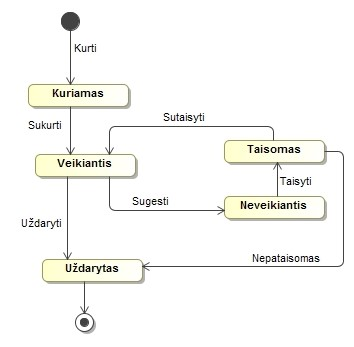
\includegraphics[scale=0.5]{img/Pav/TinklalapioBusena}
	\label{uml:29}
	\caption{Tinkalalio būsena}
\end{figure}

Vartotojas gali būti: lankytojas, vartotojas, ieškantis, turintis informaciją, nepatenkintas, radęs informaciją, norintis naudotis spec. funkcijas, neprisijungęs, neturintis paskyros, nenorintis kurtis, kuriantis paskyrą, turintis paskyrą, prisijungęs, naudojantis spec. funkcijas, patenkintas. Pačioje pradžioje asmuo atsidaręs tinklalapį yra tik lankytojas, kai jis naudojasi juo tampa vartotoju. Jeigu vartotojas ieško informacijos jis tampa ieškantis. Kai turi informaciją (tampa turinčiu informaciją), jeigu jis yra nepatenkintas informacija, jis tampa nepatenkintas ir išeina iš tinklalapio. Tačiau jei vartotojas randa informaciją, jis tampa radęs informaciją ir jeigu ieško daugiau informacijos grįžta atgal į vartotoją. Kai randa visą informaciją, kurios norėjo tampa patenkintu. Tačiau jeigu vartotojas nori ne vien ieškoti informacijos tada jis tampa norintis naudotis spec. Funkcijas. Jeigu jis nėra prisijungęs prie savo paskyros (yra neprisijungęs) jis gali būti dviejų būsenų arba neturintis paskyros, tada jeigu nori susikurti paskyrą jis tampa kuriantis paskyrą ir po to būna prisijungęs, arba jeigu nenori kurtis, jis tiesiog išeina iš tinklalapio. Tačiau neprisijungęs vartotojas gali ir turėti paskyrą, tada jis gali prisijungti prie jos ir tapti prisijungusiu. Taip prisijungę asmenys gali naudotis spec. funkcijomis ir taip tampa patenkinti.

\begin{figure} [H]
	\centering
    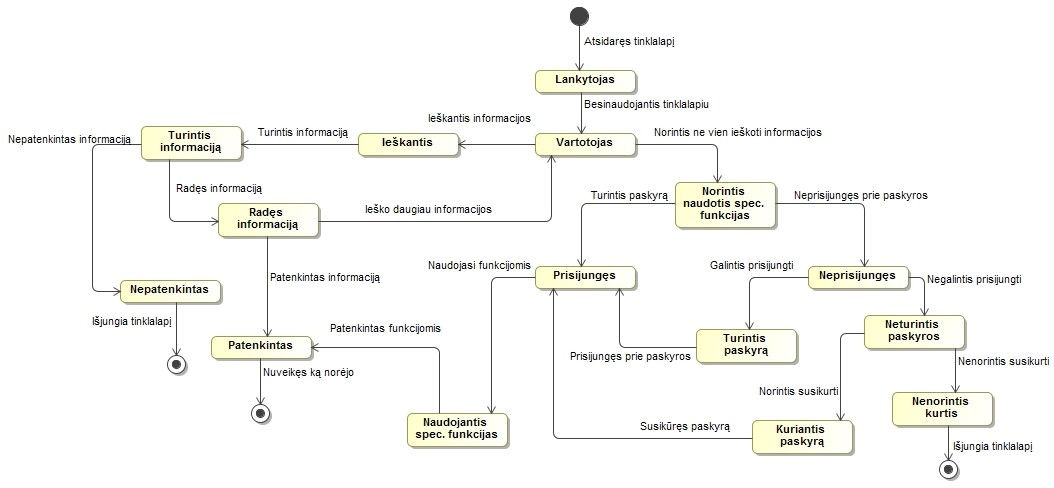
\includegraphics[scale=0.45]{img/Pav/VartotojoBusena}
	\label{uml:30}
	\caption{Vartotojo būsena}
\end{figure}

\section{Programų sistemos komponentai}
 
Šiame skyriuje pateikiamas sistemos komponentų suskirstymas naudojant UML komponentų diagramas. Komponentai skirtomi pagal duomenų judėjimo kryptis atsižvelgiant į jų funkcionalumą, nes taip aiškiausiai ir logiškiausiai atpindimos tinkalapio dalys ir jų funkcijos - skirtymas pagal technologijas arba prieigas neleido pakankamai gerai dekomponuoti sistemą ir apibrėžti jos veikimą. Kai kurie sudėtingesni komponentai norint patikslinti funkcionalumą išskirstyti į mažesnius komponentus.



\begin{figure}[H]
\centering
    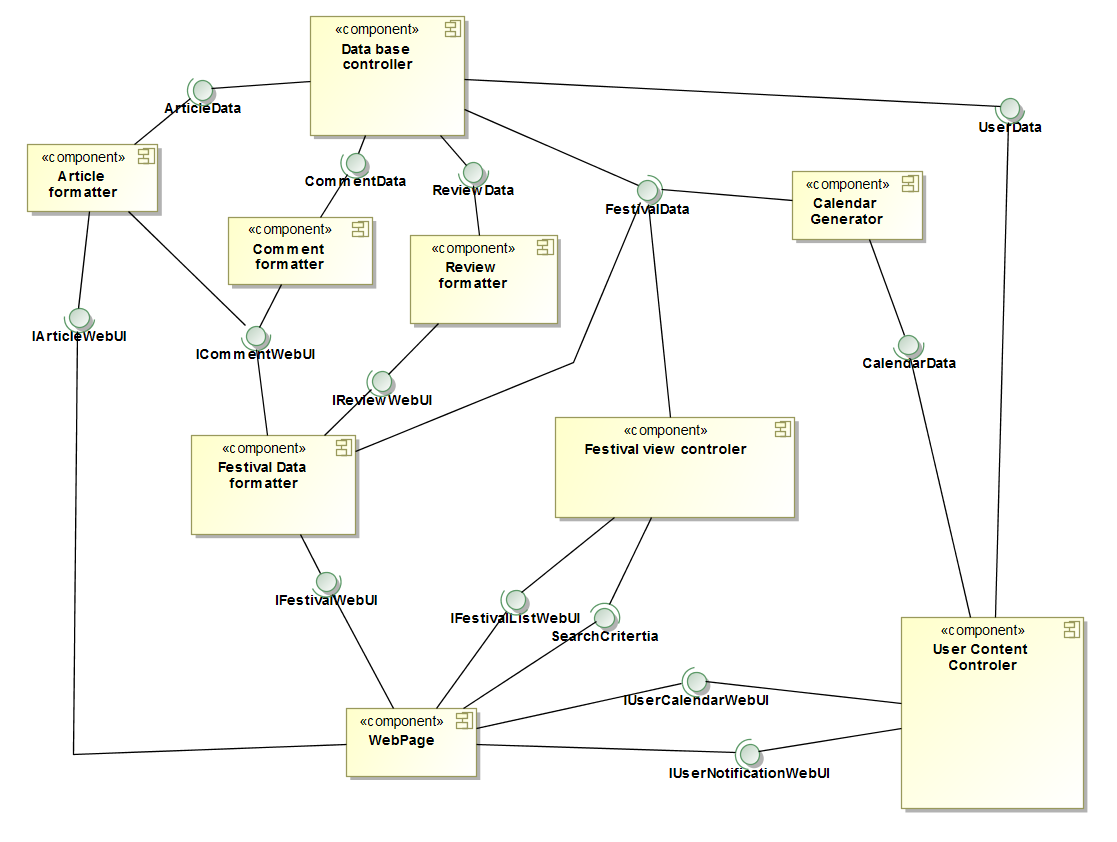
\includegraphics[scale=0.55]{img/PSI3/DataToWeb.PNG}
	\label{mantas:1}
	\caption{Duomazės - tinklalapio ryšių komponentų diagrama}
\end{figure}
Šioje diagromoje vaizduojama kaip duomenys iš duombazės pateikiami tinkalapiui.
 \textit{Data base controller} pagalba iš duomenų bazės gaunami komentarų duomenys naudojant \textit{CommentData} interfeisą, straipsnių duomenys naudojant \textit{ArticleData} intereisą, atsiliepimų duomenys (vertinimai žvaigždutėmis ir tek tu) pasitelkus \textit{ReviewData} interfeisą, duomenys apie festivalius \textit{FestivalData} interfeisu, vartotojų duomenys panaudojant \textit{UserData} intereisą.
 \textit{Comment Formatter} gautus duomenis pavercia web vartotojo sąsaja ir perduoda kaip \textit{ICommentWebUI} intereisą.
 \textit{ArticleFormatter} gautus straipsnių duomenys paverčia HTML5 dokumentu, susieja straipnius su komentarais apie juos pateikia kaip \textit{IArticleWebUI}.
 \textit{Review Formatter} komponentas paverčia per \textit{ReviewData} gautus atsiliepimų duomenis web interfeisu \textit{IReviewWebUI}.
 \textit{Fesival data formatter} komponentas atsakingas už kiekvieno individualaus festivalio puslapio išvaizdos interfesio \textit{IFestivalWebUI} generavimą naudojant komentarų ir atsiliepimų gautus Web interesus ir festivalio duomenis.
 \textit{Fesival view controller} naudodamas iš tinklalapio gautus paieškos kriterius kaip \textit{SearchCriteria} intereisą ir duomenis apie fesivalius sukuria fesivalių sąrašo interfesisą \textit{IFestivalListWebUI}.
 Festivalio duomenys naudojami \textit{Calendar Generator} komponento generuoti festivalių kalendorių ir perduoti jį kaip \textit{CommentData} interfeisu \textit{User Contnent Controller} kuris atsakingas už kalendoriaus ir asmeninių pranešimų apie ateinančius festivalius web vartotojų sąsajų interefesių perdavimą pagrindiniam tinkalalpiui. 

 \begin{figure}[H]
\centering
    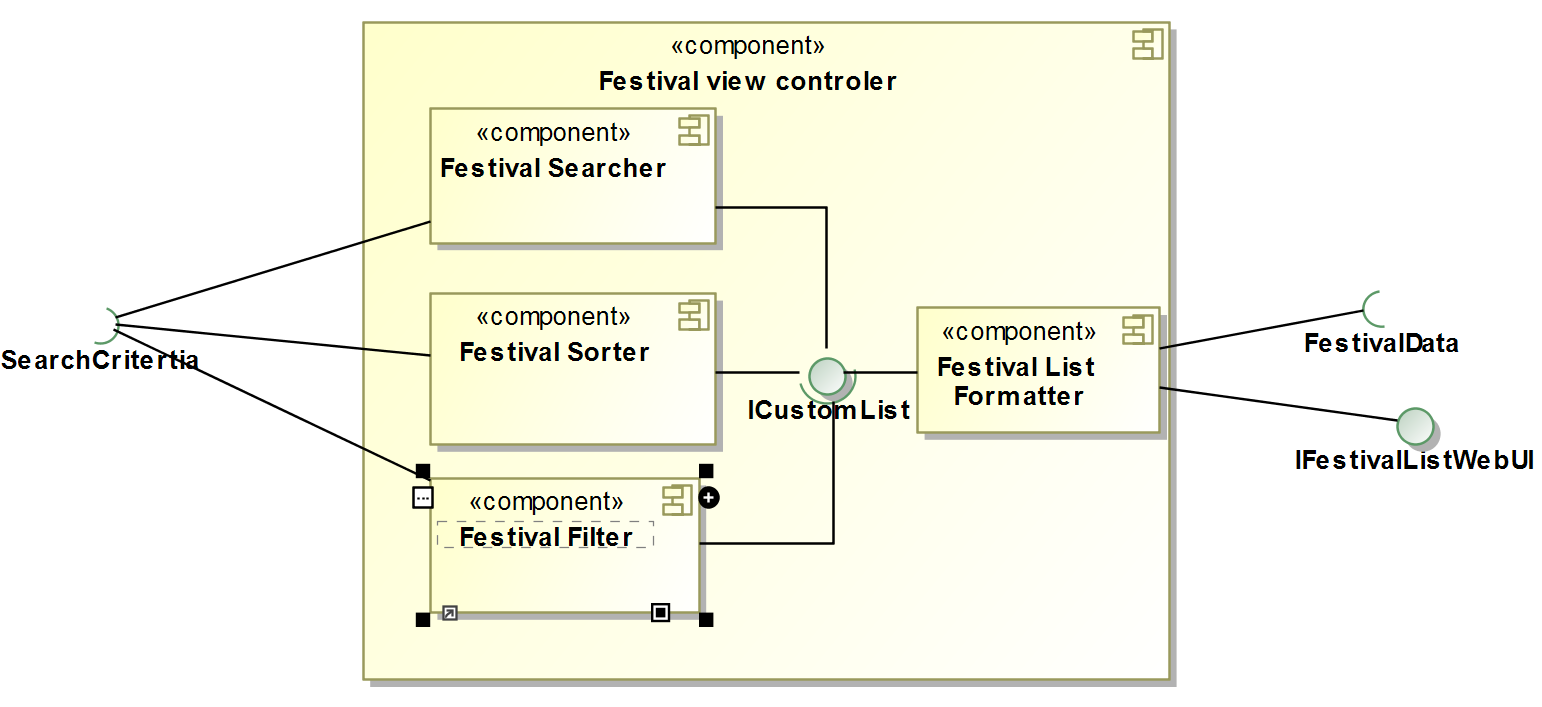
\includegraphics[scale=0.4]{img/PSI3/FestivalisViewController.PNG}
	\label{mantas:2}
	\caption{Detalizuota festivalių sarašo geravimo komponentų diagrama}
\end{figure}

\textit{Festival view controller} detalizuotoje diagramoje pavaizduoti komponentai \textit{Fesival Sorter}, \textit{Festival Searcher} ir \textit{Fesival Filter} atsakingus už festivalių sąrašo tvarkymą. Visi kompontai naudodama \textit{SearchCriteria} interfeisą paramentrų gavimui ir \textit{ICustomList} interfeisą rezultato gražinimui. Komponentas \textit{Festival List Controller} ataskingas už festivalių sarašo formavamimą naudojant \textit{FestivalData} interfeisą ir pateikia web vartotojo sąsają textit{IFestivalListWebUI}. 

\begin{figure}[H]
\centering
    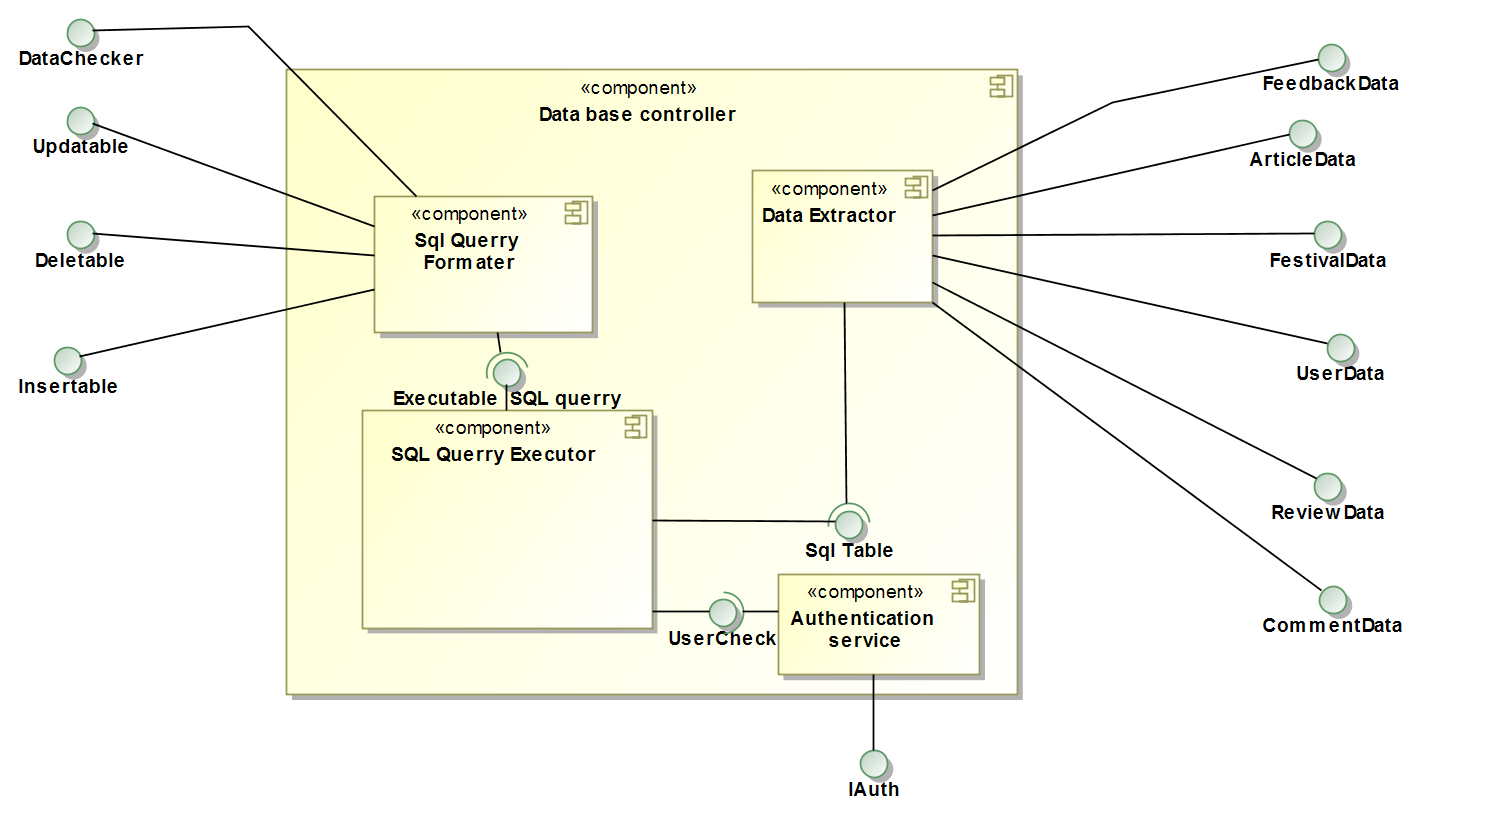
\includegraphics[scale=0.5]{img/PSI3/DataBaseController.PNG}
	\label{mantas:4}
	\caption{Detalizuota festivalių sarašo geravimo komponentų diagrama}
\end{figure}

Detalizuotoje \textit{Data base controller} komponentų diagramoje vaizduojame kaip formuojamos ir vykdomos SQL duomenų 
bazės užklausos. \textit{Sql Querry Formatter} komponentas teikia iterfesius reikalingus formuoti pagrindines duomenų bazės 
operacijas - Insert,Delete, Update ir Select ir naudodamas \textit{Executable SQL querry} interfeisą formuoja užklausas 
duomenų bazei. \textit{SQL querry executor} komponetas įvykdo gautas užklausas ir pateikia rezultatus kaip textit{SQL Table
}interfeisą. Taip pat šis komponentas tikrina ar suvesti vartotojo duomenys teisingi, gaudamas ir grąžindamas rezultatą per
{UserCheck} iterfeisą, kurį naudoja \textit{Authentication service} komponentas teikdamas \textit{IAuth} interfeisą. Komponentas
\textit{Data Extractor} išanalizuoja gautus duomenis, teikdamas įvairius duomenų perdavimo intereisus.

\begin{figure}[H]
\centering
    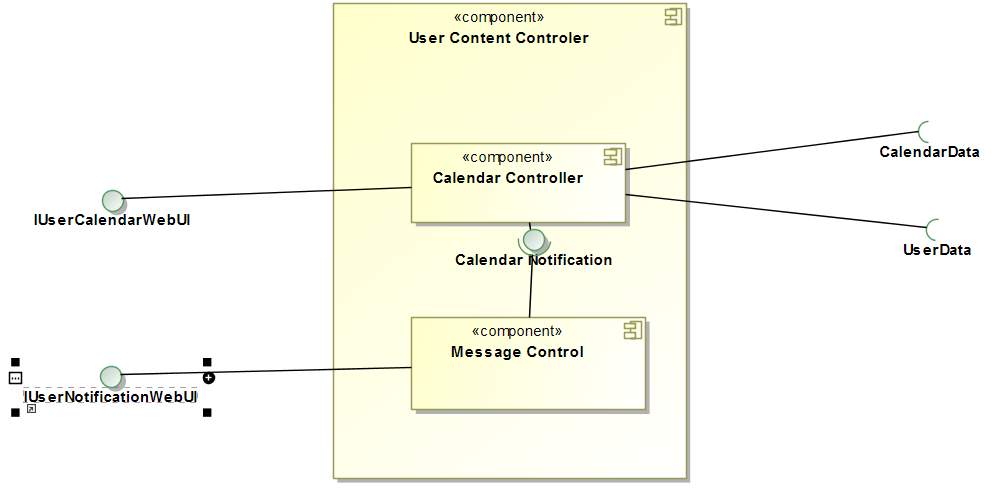
\includegraphics[scale=0.5]{img/PSI3/UserContentController.PNG}
	\label{mantas:5}
	\caption{Detalizuota festivalių sarašo geravimo komponentų diagrama}
\end{figure}

Detalizuotoje \textit{User Controller diagramoje} aprašoma kaip veikia tinkalalapyje esantis kalendorius. \textit{Calendar 
controller} gautus duomenis apie vykstančių festivalių datas ir vartotojus sujungia į vartotojo kalendorių ir pateikia kaip
\textit{IUserCalendarWebUI} intereisą tinklalapiui. Taip pat šis komponentas turi \textit{Calendar Notification} interfeisą 
kurį naudoja \textit{Message Control} komponentas atsakingas už vartotojo informavimą apie ateinančius festivalius. Žinutės 
tinklaslapiui perduodamos \textit{IUserNotificationWebUI}.


 \begin{figure}[H]
\centering
    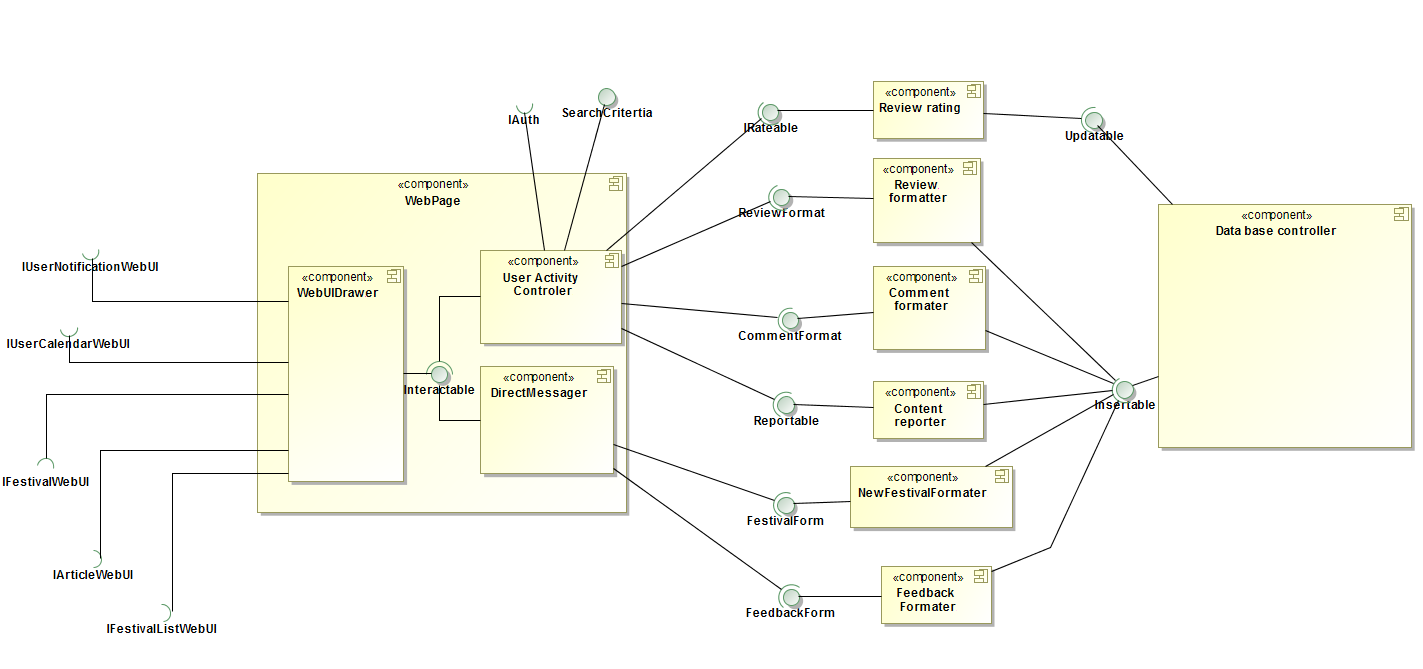
\includegraphics[scale=0.4]{img/PSI3/WebPage.PNG}
	\label{mantas:3}
	\caption{Detalizuota festivalių sarašo geravimo komponentų diagrama}
\end{figure}

Viršuje esančioje diagramoje vaizduojama kaip tinklalapio WebPage komponentas ir jo sąveika su duomenenų baze.
\textit{WebDrawer} komponentas naudodamas įvarius \textit{webUI} interfesus kuria tinklalapio grafinį vaizdą ir turi interfeisą \textit{Interactable} kuris
leidžia bendrauti su komponentas atsakingais už vartotojų veiklos tinklalapyje perdavimą duomenų bazei. \textit{User activity controller} 
perduoda prisijungūsių vartotojų sąveikas - įvertinimus,atsiliepimus, komentarus, pranešimus apie netinkamą turinį kompontams kurie 
atsakingi už šių pranešimų performulavimą duomenų bazei suprantama kalba. Analogiškai vyksta ir su \textit{Direct Message} komponentu, tik ten perduodamas nebutinai prisijungūsių vartotojų turinys pranešimai apie festivalius ir atsielimai apie tinklalapį. 
\section{Komponentų išskirstymas tinkle}
Pateikiama diegimo diagrama, kurioje pavaizduota, kaip festivalių informacinė sistema bus išskirstyta aparatinėje įrangoje. 
\begin{figure}[H]
\centering
    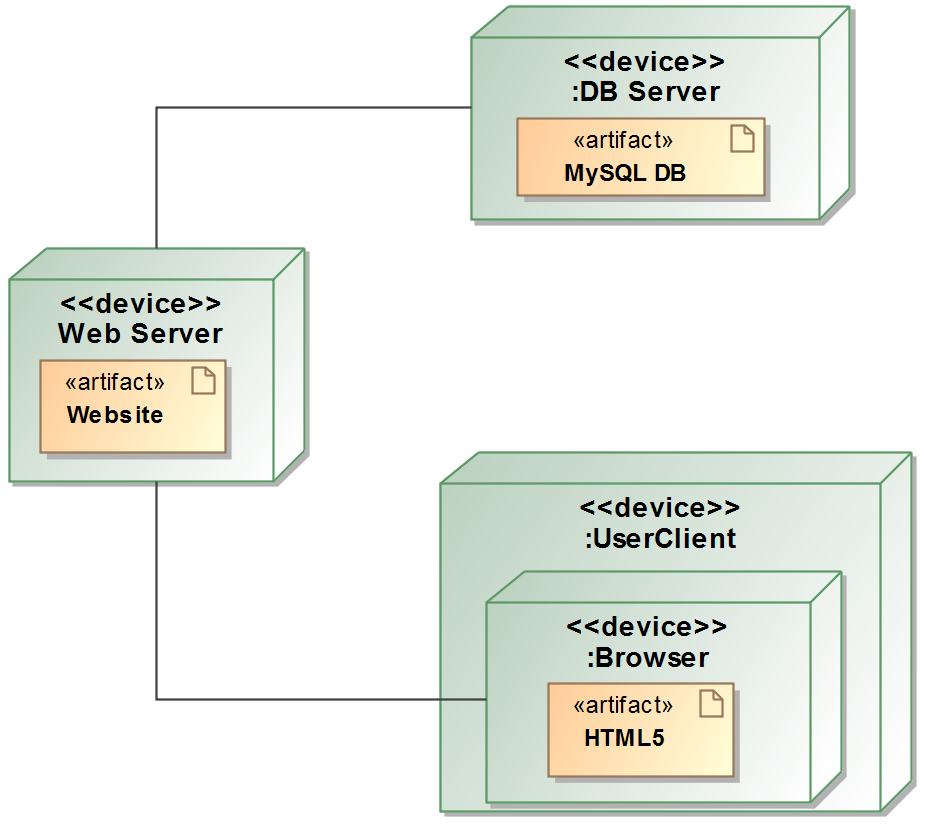
\includegraphics[scale=0.5]{img/PSI3/deploy.PNG}
	\label{uml:22}
	\caption{Komponentų išskirstymas tinkle}
\end{figure}
Informacija yra saugoma duomenų bazės serveryje (\textit{DB Server}), kuriame yra \textit{MySQL} duomenų bazė. Tinklalapis (\textit{Website}), veikiantis žiniatinklio serveryje (\textit{Web Server}), tvarko ir apdoroja informaciją, saugomą duomenų bazėje. Vartotojas pasiekia tinklalapį per naršyklę, palaikančia HTML5. Naršyklę turi būti instaliuota įrenginyje su interneto prieiga.



\sectionnonum{Literaturos sarašas}
\begin{itemize}
\item http://manofestivalis.lt/
\item https://www.facebook.com/ManoFestivalis.lt/?fref=ts
\item https://www.e-tar.lt/portal/lt/legalAct/TAR.5368B592234C/lGOrBAvuZc (Lietuvos Respublikos asmens duomenu teisines apsaugos istatymas)
\item https://www.esparama.lt
\item https://www.vmi.lt/ (2\% nuo pajamu mokescio parama)
\item http://www.hostingas.in/
\item http://jobarnesonline.com/free-facebook-ad-spend-calculator/
\item https://www.tutorialspoint.com/uml/uml\_2\_overview.htm
\item http://www.mif.vu.lt/\textasciitilde karolis/PSI1.html
\end{itemize}

%\appendix  % Priedai
% Prieduose gali buti pateikiama pagalbine, ypac darbo autoriaus savarankiškai
% parengta, medžiaga. Savarankiški priedai gali buti pateikiami ir
% kompaktiniame diske. Priedai taip pat numeruojami ir vadinami. Darbo tekstas
% su priedais susiejamas nuorodomis.

%Citavimo pavyzdžiai: cituojamas vienas šaltinis \cite{PvzStraipsnLt}; cituojami
%keli šaltiniai \cite{PvzStraipsnEn, PvzKonfLt, PvzKonfEn, PvzKnygLt, PvzKnygEn,
%PvzElPubLt, PvzElPubEn, PvzMagistrLt, PvzPhdEn}.
%
%
%\subsubsection{Skirsnis}
%\subsubsubsection{Straipsnis}
%\subsubsection{Skirsnis}%

\end{document}
